% !TeX root = ../main.tex
% Add the above to each chapter to make compiling the PDF easier in some editors.

\chapter{Literature Review}\label{chapter:literature_review}

\section{Geo-based Content Sharing}
In typical networks (such as social networking etc.), the content is shared among users irrespective of their geographic location. There are a number of advantages to this such as:

\begin{itemize}
  \item High availability
  \item Reliability
  \item a large amount of content.
\end{itemize}

However, there are some disadvantages to such networks such as:

\begin{itemize}
  \item A connected network is needed for the services to work, so in case the connectivity is lost, normally the content is also gone.
  \item The system/network is prone to censorship
\end{itemize}

Geo-based content sharing has been introduced to make the information/content more customized based on the user location such as chatting with people nearby, posting in a local message board etc. There are two types of networks used for Geobased content sharing: \emph{Connected Systems/Networks} and \emph{Peer-to-Peer Systems/Networks}.

\subsection{Connected Systems/Networks}
Connected Network is a connected set of devices where each device is connected to one or more other devices in the network. One common setting is the server-client architecture, which clients connect to servers to access resources. Since server provides resources, there can be different kinds of servers such as file server, web server, application server etc. A very basic example of such architecture is world wide web (www) where users (clients) can access websites, files etc. In such networks, there is a very high probability that the message is delivered to the desired device.

Connected Networks enable the service providers to provide a very reliable service. Social media applications/websites, chatting applications, and e-commerce application etc. use connected networks to provide services to their clients.

\subsection{Peer-to-Peer Systems/Networks}
Peer-to-Peer Networks don't rely on the network infrastructure to relay information, so they can work even when there is no server/central controller or no pre-determined path between the sender and receiver. A key property of such systems is that they do not rely on infrastructure nodes or cloud services to ensure data availability but rather replicate content items within a defined geographic area among mobile nodes in a device-to-device (peer-to-peer) fashion. While this operation does not require infrastructure network access—and thus limits dependencies as well as vulnerability to third-party actions such as traceability or censorship—it comes at the cost of unpredictability: there is no guarantee that content “posted” to a defined geographic area will remain available. We refer to this property as best-effort (probabilistic) content sharing \cite{geo-based-content-sharing}.

Below are a few systems/concepts utilizing this methodology/concept:
\begin{itemize}
  \item Hovering Information \cite{Castro2009}
  \item Locus \cite{Thompson:2010:LLD:1859934.1859945}
  \item Ad Loc \cite{Corbett2006ADL}
  \item Floating Content \cite{floating-content}
\end{itemize}

\subsubsection{Hovering Information \cite{Castro2009}}
Hovering information is a concept characterizing geo-localized self-organizing information responsible to find its own storage on top of a highly dynamic set of mobile devices. This information is attached to a geographical point, called the \textit{anchor location}, and to its vicinity area, called \textit{anchor area}. The main requirement of a single piece of hovering information is to keep itself stored at some specified location (\textit{anchor location}) despite the unreliability of the device on which it is stored. Whenever the mobile device, on which the hovering information is currently stored, leaves the area around the specified storage location, the information has to hop - ”hover” - to another device.
Hovering information uses mechanisms such as active hopping, replication, and dissemination among mobile nodes. It does not rely on any central server. To achieve this purpose, two main algorithms are used, which are, the \textit{Attractor point} algorithm and the \textit{Broadcast} algorithm. Below is a short description of both of these algorithms:
\begin{itemize}
  \item \textbf{Attractor Algorithm}: The anchor location acts as an attractor for the hovering information attached to it. The purpose of this algorithm is to keep the hovering information alive in its \textit{anchor area} as long as possible.
  \item \textbf{Broadcast Algorithm}: The hovering information broadcasts/replicates itself to all the nodes in the communication range. The purpose of this algorithm is to provide better availability of the information, however, it uses more memory and network resources.
\end{itemize}

\subsubsection{Locus \cite{Thompson:2010:LLD:1859934.1859945}}
Locus, a location-based data overlay for DTNs. Locus keeps objects at specific physical locations in the network using whatever devices currently are nearby. Nodes copy objects between themselves to maintain the locality of data. Location utility functions prioritize objects for replication and enable location-based forwarding of data look-ups. As a first-of-its-kind application, Locus is compared against other possible replication policies and shown to achieve query success rates nearly 4 times higher than other approaches.
As a mobile device moves through the network, it creates new data periodically. Each piece of data created has a timestamp (also known as creation time), an application specific type indicator and the current location, which becomes the \textit{home location} for the newly created data. The location-based design requires that the devices have a GPS or any other mechanism to capture the current location. The main goal is to keep the data as close as possible to the location it was sensed so that it can be easily found later.
To access data in Locus, nodes forward query messages to the physical regions in which the node is interested. Every query message contains a \textit{target location} (location of interest), and the type of data needed. Any intermediate node, that receives the query, can respond if it contains any data with \textit{home location} matching the \textit{target location}. Once matching data is found, a response message containing the data is sent back to the original requesting node.

\subsubsection{AD LOC \cite{Corbett2006ADL}}
AD LOC is an infrastructure-free, localized, persistent and asynchronous platform for collaboratively annotating the physical environment with \textit{notes}. Below are some characteristics of the notes:

\begin{itemize}
  \item \textbf{Localized}: notes are specific to physical locations.
  \item \textbf{Persistent}: notes remain in the environment.
  \item \textbf{Asynchronous}: notes and published and consumed without the need for both the consumers and publishers to be available at the same time.
  \item \textbf{Collaborative}: anyone can publish or read any note.
  \item \textbf{Infrastructure-free}: no servers or internet connections.
\end{itemize}

As users with mobile devices pass through locations, they automatically receive notes published there and makes them available to other users. As users leave, their cached notes can be transferred to other devices remaining at the location.


\subsubsection{Floating Content \cite{floating-content}}
Floating content is an ephemeral content sharing service, solely dependent on mobile devices in the vicinity using principles of opportunistic networking. The net result is a best effort service for floating content in which: 1) information dissemination is geographically limited; 2) the lifetime and spreading of information depend on interested nodes being available; 3) traffic can only be created and caused locally; and 4) content can only be added, but not deleted. Floating Content is discussed in more details \hyperref[section:floating-content]{\emph{later in the chapter}}.

\subsection{Delay Tolerant Networking (DTN)}
Delay-tolerant Networking (DTN) enables communication in sparse mobile ad-hoc networks and other challenged environments where traditional networking fails and new routing and application protocols are required. Past experience with DTN routing and application protocols has shown that their performance is highly dependent on the underlying mobility and node characteristics \cite{keranen-theone}. The basic idea behind DTN is to communicate data/messages from the source to the destination without having complete network connectivity. The path from the source to the destination is unknown due to the unconnected nature of the network. In such networks, each node store the messages it receives and forwards it to the next node it comes in contact with. The message may or may not reach its final destination.\newline
DTNs are also known \textit{Opportunistic Networks} due to the fact that the nodes connect to each other and transfer message as soon as they get the opportunity (when they come in vicinity of each). Below are a few characteristics of DTNs:
\begin{enumerate}
  \item \textbf{Mobility}: DTN is based on the concept of mobile nodes which enables the flow of information. Unlike traditional networks, node mobility to required to transfer data.
  \item \textbf{Dynamic}: Since the nodes are mobile, old nodes leave and new nodes connect to the network, making it a very dynamic network.
  \item \textbf{Limited Resources}: DTNs utilized mobile devices/nodes which have lesser resources than a normal computer. Such resources include processing power, memory and more importantly battery/energy.
\end{enumerate}

\newpage
\section{The ONE Simulator}
\subsection{Introduction}
The ONE is an Opportunistic Network Environment simulator \cite{the-one} which provides a powerful tool for generating mobility traces, running DTN messaging simulations with different routing protocols, and visualizing both simulations interactively in real-time and results after their completion \cite{the-one-ari}.

The ONE simulator was originally developed in Aalto University in the SINDTN \cite{sindtn} and CATDTN projects supported by Nokia Research Center (Finland). It is now maintained in by Aalto Univerity in cooperation with the Technical University of Munich.\newline

The ONE Simulator has the following capabilities:
\begin{itemize}
  \item Message Generation at different intervals.
  \item Node Movement using different movement models such as Random Walk, Mapbased movement etc.
  \item Routing messages between nodes using different types of routers such as Epidemic Router, First Contact Router etc.
  \item Graphical User Interface (GUI) for visualizing nodes movement, message creation and message passing in real time.
  \item Report Generation for different purposes such as Message Delivery Report etc.
  \item A batch mode where the app can be run without a GUI.
\end{itemize}

Figure ~\ref{fig:onesimulatorenvironment} illustrates the different components of the ONE (Opportunistic Network Environment) simulator and how they work together. Below is a short explanation of each component.

\begin{itemize}
  \item \textbf{Simulation Engine} is the main component that drives the ONE simulator. In other words, it is the controller of the ONE simulator. It is responsible for handing event generation, routing and report generation, to name a few.
  \item \textbf{Event Generators} are responsible for generating different types of events. One simple example is the generation of a message by a node/host.
  \item \textbf{Movement Models} specify the movement patterns for the hosts. There are a number of movements models that we can use. One example would be the map based movement, where the hosts follow the map (or a specific route on the map).
  \item \textbf{Routers} are responsible for the routing of the messages between nodes. An example would be the DirectDelivery router, which delivers the message only to the final recipient (in other words, it does not use any intermediate node for transferring messages).
  \item \textbf{Results/Reporting} is responsible for storing the different simulation data (such as connectivity between different hosts, the average life of a message etc) on the filesystem. These files are later used either for visualization or for verification/inference of results.
\end{itemize}
\begin{figure}[h]
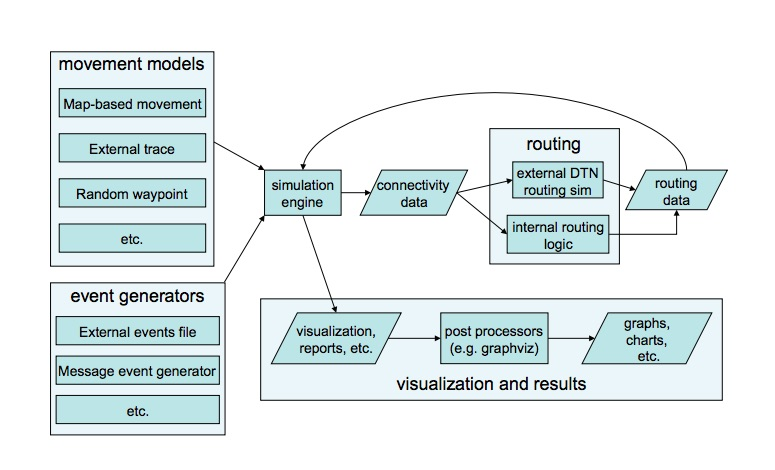
\includegraphics[scale=0.5]{./figures/one}
\caption{Overview of the ONE simulation Environment \cite{keranen-theone}}
\label{fig:onesimulatorenvironment}
\end{figure}

\subsection{Compilation}
ONE can be compiled from the source code using both Command Line and Eclipse. However, we will discuss only the command line. The ONE source contains \textit{compile.sh} and \textit{compile.bat} for compilation on the Linux/Unix and Windows Platform respectively.
\newline
\subsection{Running}
Just like Compilation, ONE can be run from both Command Line and Eclipse. However, we will discuss only the command line.

\begin{lstlisting}[language=bash]
./one.sh [-b repetitionCount] [configuration-files]
./one.bat [-b repetitionCount] [configuration-files]
\end{lstlisting}

\textbf{-b} is an optional parameter. Start the ONE simulator in batch (non-UI) mode. \textit{repetitionCount} specifies the number of times the simulations need to repeat. If not defined, the ONE simulator starts in UI mode.\newline
\textbf{configuration-files} is an optional parameter, where we can specify a number of configuration files separated by space. The simulation parameters are read from these files. Files specified later override values in the earlier config files.\newline

\subsection{Configuration}
\label{one:configuration}
One of the amazing features of ONE is that there is no need for changing the code and recompilation if need to change any configuration (such as changing the number of hosts, changing the movement models etc.). All of these can be done in the configuration files which are ordinary text files. By default, the ONE simulator uses \textbf{default\_settings.txt} configuration file. However, additional configuration files can also be passed.

Configuration files contain key-value pairs. Below is the basic syntax for most of these pairs:
\begin{lstlisting}[language=bash]
Namespace.key = value
\end{lstlisting}

Both \textit{Namespace} and \textit{key} follow the camelCase and are case sensitive. \textit{value} can be numeric, boolean, strings, comma-separated values, value filling and reference to other files. Numeric values can also use the suffixes \textit{k} for Kilo, \textit{M} for Mega and \textit{G} for Giga.

\subsection{Components}
\subsubsection{Host Group}
Host Groups represents a collection of hosts with the same configuration such as Movement Model etc. In other words, similar nodes are grouped in a Host Group. Theoretically, each host group must have a different configuration from the other host groups. All the host groups can also share configuration (such as the number of hosts etc.) which are defined under \textit{Group} namespace. However, configuration inside the specific host group takes precedence over the global \textit{Group} namespace.
\begin{lstlisting}[language=bash]
Group.nrofHosts = 20

Group1.groupID = G1
Group1.nrofHosts = 30
Group2.groupID = G2
Group3.groupID = G3
\end{lstlisting}

In the above listing, \textit{Group} defines the number of hosts (i.e. 20) for all the groups. However, \textit{Group1} overrides this property and sets the number of hosts to 30. So, now we have three groups where \textit{Group1} has 30 hosts while \textit{Group2} and \textit{Group3} have 20 hosts each.

\subsubsection{Movement Models}
Movement Models dictate the node movements in the simulation. A number of Movement Models come packaged with the ONE simulator such as \textit{Map based Movement}, \textit{Shortest Path Map based Movement}, \textit{Random Waypoint}, \textit{External Movement} and \textit{Stationary Movement}. \textit{Map based Movement} has further types of movements such as \textit{Car Movement} and \textit{Map Route Movement} etc.
\begin{lstlisting}[language=bash]
Group.movementModel = MapbasedMovement
Group1.movementModel = RadomWaypoint
\end{lstlisting}

In the above listing, we are setting the movement type for all the groups to \textit{MapbasedMovement}, however, \textit{Group1} is overriding and setting it to \textit{RandomWaypoint}.

\subsubsection{Routing}
Routing Module is responsible for handling the transfer (routing) of messages between hosts. ONE simulator one passive and a number of active routers. A passive router is used for interacting with other DTNs or dummy nodes. The active routers implement the well-known routing algorithms for DTN such as \textit{Epidemic}, \textit{Spray and Wait}, \textit{First Contact}, \textit{Direct Delivery}, \textit{Prophet}, \textit{Prophet V2}, \textit{Life}, \textit{Wave}, \textit{MaxProp} and \textit{Floating Content}.
\begin{lstlisting}[language=bash]
Group.router = EpidemicRouter
Group2.router = DirectDeliveryRouter
\end{lstlisting}

In the above listing, \textit{EpidemicRouter} is used for all the groups except \textit{Group2} which is using the \textit{DirectDeliveryRouter}.


\subsubsection{Value Filling}
Value Filling is used to dynamically fill the value during run-time. The main purpose is to use the value of a variable during run-time. To use value-filling, we put the key name as value surrounded by %% such as %%keyName%%. Below is an example:
\begin{lstlisting}[language=bash]
MovementModel.warmup = %%Reports.warmup%%
\end{lstlisting}

In the above listing, we are setting up the warmup for \textit{MovementModel} to be the same as the warmup used for \textit{Reports}.

\subsubsection{Run Indexing}
There are times when we want to run a number of simulations for different permutations of the configuration such as varying number of hosts, varying size of the message etc. One solution would be to create different configurations and write a script passing the desired configuration for each run. However, it is not a maintainable solution if we have a different number of permutations (changing 3 values each for two different parameters). The ONE (Opportunistic Network Environment) simulator solves this problem by using run indexing. Run indexing allows us to change configuration during run-time by providing the same configuration file;  containing a set of semi-colon separated values surrounded by braces ([]) for the desired key(s).

\begin{lstlisting}[language=bash]
Reports.warmup = [0; 100; 200; 300]
\end{lstlisting}

In the above listing, the first run will use the value 0, next one will use the value 100 and so on. In case the values are less than the total number of simulations, the indexes wrap around (loops back to the start of the array when there is no further item to read).
\newpage
\section{Floating Content}
\label{section:floating-content}
Floating content is an ephemeral content sharing service, solely dependent on the mobile devices in the vicinity using principles of opportunistic networking. The net result is a best effort service for floating content in which: 1) information dissemination is geographically limited; 2) the lifetime and spreading of information depend on interested nodes being available; 3) traffic can only be created and caused locally; and 4) content can only be added, but not deleted \cite{floating-content}.

In Floating Content, a message (a text message, an image, etc.) deemed to be of interest to other people at a certain area is tagged with geographical coordinates of that area. This area is referred to as the anchor zone of the message \cite{floating-content-1}. Each message has two main properties namely \textit{Center} and \textit{Availability/anchor zone}. For the sake of simplicity, the anchor zone is defined as a circle with a radius. In short, floating messages can be relayed to other nodes inside the anchor zone. Every time a copy of the message is made, the anchor zone properties are copied to make sure that the copied message has the same anchor zone as the original message.

Whenever a message is generated, it is assigned an anchor zone (identified by a radius and the node's current location). The message is transferred to other nodes in the anchor zone. Whenever a node moves out of the anchor zone, it may delete its copy of the message or keep it until first interaction with another node depending on the configuration.
\subsection {System Operation \cite{Ott2011FloatingCI}}
A node generates an information item/message \textit{I} of size \textit{s(I)} with a certain lifetime (\textit{TTL}) and assigns an anchor zone with center \textit{C} and two radii \textit{a} and \textit{r}. The difference between \textit{a} and \textit{r} is listed below:

\begin{enumerate}
  \item \textbf{Availability zone (\textit{a})}: \textit{a} defines the availability zone of the item, which is the region/zone within which the item \textit{I} is still kept around with a limited probability. In other words, this is the region/zone where the item \textit{I} can exist.
  \item \textbf{Replication zone (\textit{r})}: \textit{r} defines the replication zone of the item, which is the region/zone within which the node always try to replicate the item to any other node it encounters.
\end{enumerate}
\vspace{3mm}
If two nodes \textit{A} and \textit{B} meet in the anchor zone (or replication zone to be specific) and \textit{A} has a copy of \textit{M} while \textit{B} does not, then \textit{A} replicates message \textit{M} to \textit{B}. Theoretically, every node in the anchor zone should have a copy of the message. However, practically it is not a possibility due to limited storage of the nodes.
\vspace{3mm}
Let us explain the whole phenomenon with an example:
Assuming we have 2 nodes (\textit{A} and \textit{B}). For the sake of simplicity, we assume there is only 1 item/message \textit{I} generated by \textit{A} with availability range \textit{a} and replication zone \textit{r}. Node \textit{B} now comes into the availability range \textit{a} of \textit{I}, however, nothing happens (but \textit{I} still exists on \textit{A}). Now \textit{B} enters the replication range \textit{r} or \textit{I}. When \textit{B} comes in contact with \textit{A} inside the replication zone, a copy of \textit{I} is transferred to \textit{B}. Both \textit{A} and \textit{B} keep copy of the item until they are inside \textit{a} (assuming we have unlimited storage).

\begin{figure}[h]
\centering
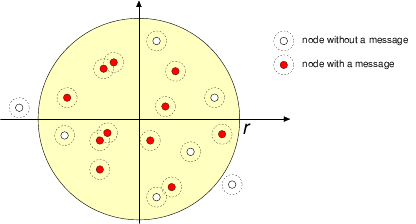
\includegraphics{./figures/anchor-zone}
\caption{Floating-Content and its anchor zone \cite{floating-content}}
\label{fig:floating-content}
\end{figure}
Figure ~\ref{fig:floating-content} shows the availability zone (\textit{a}) of the item, which is the outer circle. It also shows the replication zone (\textit{r}) of the item, which is the inner circle. Inside the inner circle (which represents \textit{r}), the item (depicted by a red dot) is copied to other nodes. Outside the inner circle and inside the outer circle (which represents \textit{a}), the item still exists but is not replicated. However, the item does not exist outside the anchor zone \textit{a}.

\subsection{Important Concepts}
The following list summarizes the important concepts:
\begin{enumerate}
  \item \textbf{interval}: The minimum time between the generation of two messages by the same node.
  \item \textbf{replication range/zone (r)}: The replication range for floating message. It is the range/zone where the message can be replicated (transferred) to other nodes.
  \item \textbf{availability range/zone (a)}: The availability range of the floating message. It is the range/zone where the message is still kept around with a limited probability.
  \item \textbf{time to live (TTL)}: The life of the floating message.
  \item \textbf{size}: The size of the floating message.
  \item \textbf{replicationPolicy}: Policy which dictates how floating messages are replicated when the node comes in contact with another node.
  \item \textbf{deletionPolicy}: Policy which dictates when floating messages are deleted.
\end{enumerate}

\subsection {Deletion Policy}
As mentioned in the above list, deletion policy dictates when the floating messages are deleted. We currently have two policies, which are explained below:
  \begin{enumerate}
    \item \textbf{Immediate}: When this policy is used, the message is deleted as soon as the node (carrying the message) leaves the anchor zone (availability zone to be specific).
    \item \textbf{Encounter}: When this policy is used, the message is deleted as soon as the node (carrying the message) comes in contact with the first node outside the anchor zone (availability zone to be specific). The advantage/use case is that the node still carries the message if it leaves the anchor zone for a short period of time (in case it does not encounter another node during that period). It is the default policy in ONE Simulator.
  \end{enumerate}

\subsection{The ONE Simulator and Floating Content}
ONE simulator has inherent support for floating content. It handles all the functionality (such as replication of messages, dropping of messages etc.) of the floating message. The following section explains the main components of the ONE simulator used for floating content:

\subsubsection{Components}
The ONE Simulator has two main components for dealing with floating content which are \textit{FloatingApplication} and \textit{FloatingContentRouter}.

\begin{itemize}
\item \textit{FloatingApplication} is responsible for generation of the messages with the floating content parameters (such as anchor, ttl etc.). FloatingApplication can be associated with any Host Group (or all the Host Groups) using the configuration file(s).
\item \textit{FloatingContentRouter} is responsible for all the routing related functionalities for the floating messages. It takes care of replication, deletion (and dropping) and prioritization of message. Replication and Deletion is performed as per the Replication and Deletion policies. Different parameters of the FloatingContentRouter can be set in the configuration file(s).
\end{itemize}

\subsubsection{Configuration}
As mentioned in the \hyperref[one:configuration]{\emph{Configuration of ONE Simulator}}, all the configurations need to be provided as configuration files containing key-value pairs. Below are some examples for setting configuration for the floating content.

\begin{lstlisting}[language=bash]
#1.
FloatingContentRouter.replicationPolicy = fifo
FloatingContentRouter.deletionPolicy = immediate
#2.
floatingApp.type = FloatingApplication
floatingApp.ttl = 300
floatingApp.destination = 0
floatingApp.messageSize = 5k
floatingApp.anchor = 200
#3.
Group.nrofApplications = 1
Group.application1 = floatingApp
Group.router = FloatingContentRouter

\end{lstlisting}
\vspace{3mm}
The above listing shows the settings needed for ONE simulator to correctly handle floating messages.
\begin{enumerate}
  \item We set different the replication and deletion policies for the floating content router (which is responsible for routing floating messages).
  \item In order to handle floating content (message), ONE simulator needs FloatingApplication.  Here we define different message properties such as time to live (ttl), message size, size of anchor zone etc.
  \item We configure each group to use the floating application and floating content router. In other words, the nodes of each group will generate, send and receive floating messages.
\end{enumerate}
